
% \section{Explanation Criteria}
% \todo{Move this section somewhere else}
% \label{sec:explanation}

% --------------------------------------
% Previous Work
% --------------------------------------

% If we are to explain a circuit in a transformer language model, we must explain how that circuit implements a certain algorithm inside the neural network. Unfortunately, this algorithm may be implemented a variable number of times, in a variable number of places, and in a manner that may or may not affect the actual output of the neural network (i.e a redundant computation).
% %\footnote{Note that by default we do not expect a neural net component to be totally redundant, however we may localize to sub-distributions in order to explain behaviors, and this may introduce redundancy.}. 
% All those factors that make the reverse engineering of such models difficult and makes the need for an empirical evaluation of the proposed explanation. 


% By avoiding the problem of inspecting the internal computations of neural nets, many prior methods fail to meet even the most basic tests of what an `explanation' of a model's behavior is (\citet{saliency}). On the other hand, imposing standards as stringent as mathematical proofs of programs that are used in other areas of computer science % for what the implementation of an algorithm means 
% is likely to prevent us from saying anything at all about the model. Internal mechanism are by nature continuous and distributed, we need to take those singular properties %too likely to be stringent at present. 
% We seek criteria that ensure explanations that capture the model internal mechanism while taking into account the continuous and distributed nature of the representation. %what the model is really computing, without restricting the set of tasks we can do interpretability on too much.

% % --------------------------------------
% % Introducing Criteria
% % --------------------------------------
% \subsection{Definitions}

% A model $M$ is a computational graph defined by %the pair \krw{can we delete the words "the pair" and just say defined by ...? in general this section reads kind of confusing to me} 
% $(V_M,E_M)$ where the vertices $V$ represent the variables of the computation and the edges $E$ the operations. A circuit $C=(V_C,E_C)$ is an induced subgraph of $M$\footnote{$V_C \subseteq V_M$ and $E_C$ contains all edges of $E_M$ connecting pairs of nodes in $V_C$}. In the following, we interchangeably refer to the set of nodes and the computational graph it induces in $M$.

% Let $\mathcal{C}_M$ denote the set of circuits in $M$. A metric is a function $\mathrm{F}: \mathcal{C}_M \longrightarrow \mathbb{R}$ that's a measure of the behavior we want to explain. For instance, $F$ can be the average difference between two logits or the predicted probability of the right token across a dataset. As a bare minimum, any circuit that is claimed to explain $M$ needs to satisfy

% \begin{itemize}
%     \item \textbf{Faithfulness}: our circuit is faithful if it includes any of the circuits that computes the task. We formulate this as $|\mathrm{F}(C) - \mathrm{F}(M)| \leq \epsilon$.
% \end{itemize}

% However, a circuit that meets the `faithful' criterion may be very inadequate as an explanation for the model's behaviour, as we find in reviewing early iterations of our work in section (\ref{sec:validation}). For $\epsilon, A \in \mathbb{R}$, we consider $C$ to be a $(\epsilon, A)$-successful explanation if it meets the three further criteria:

% \begin{wrapfigure}{r}{0.4\textwidth}
% \begin{center}
% 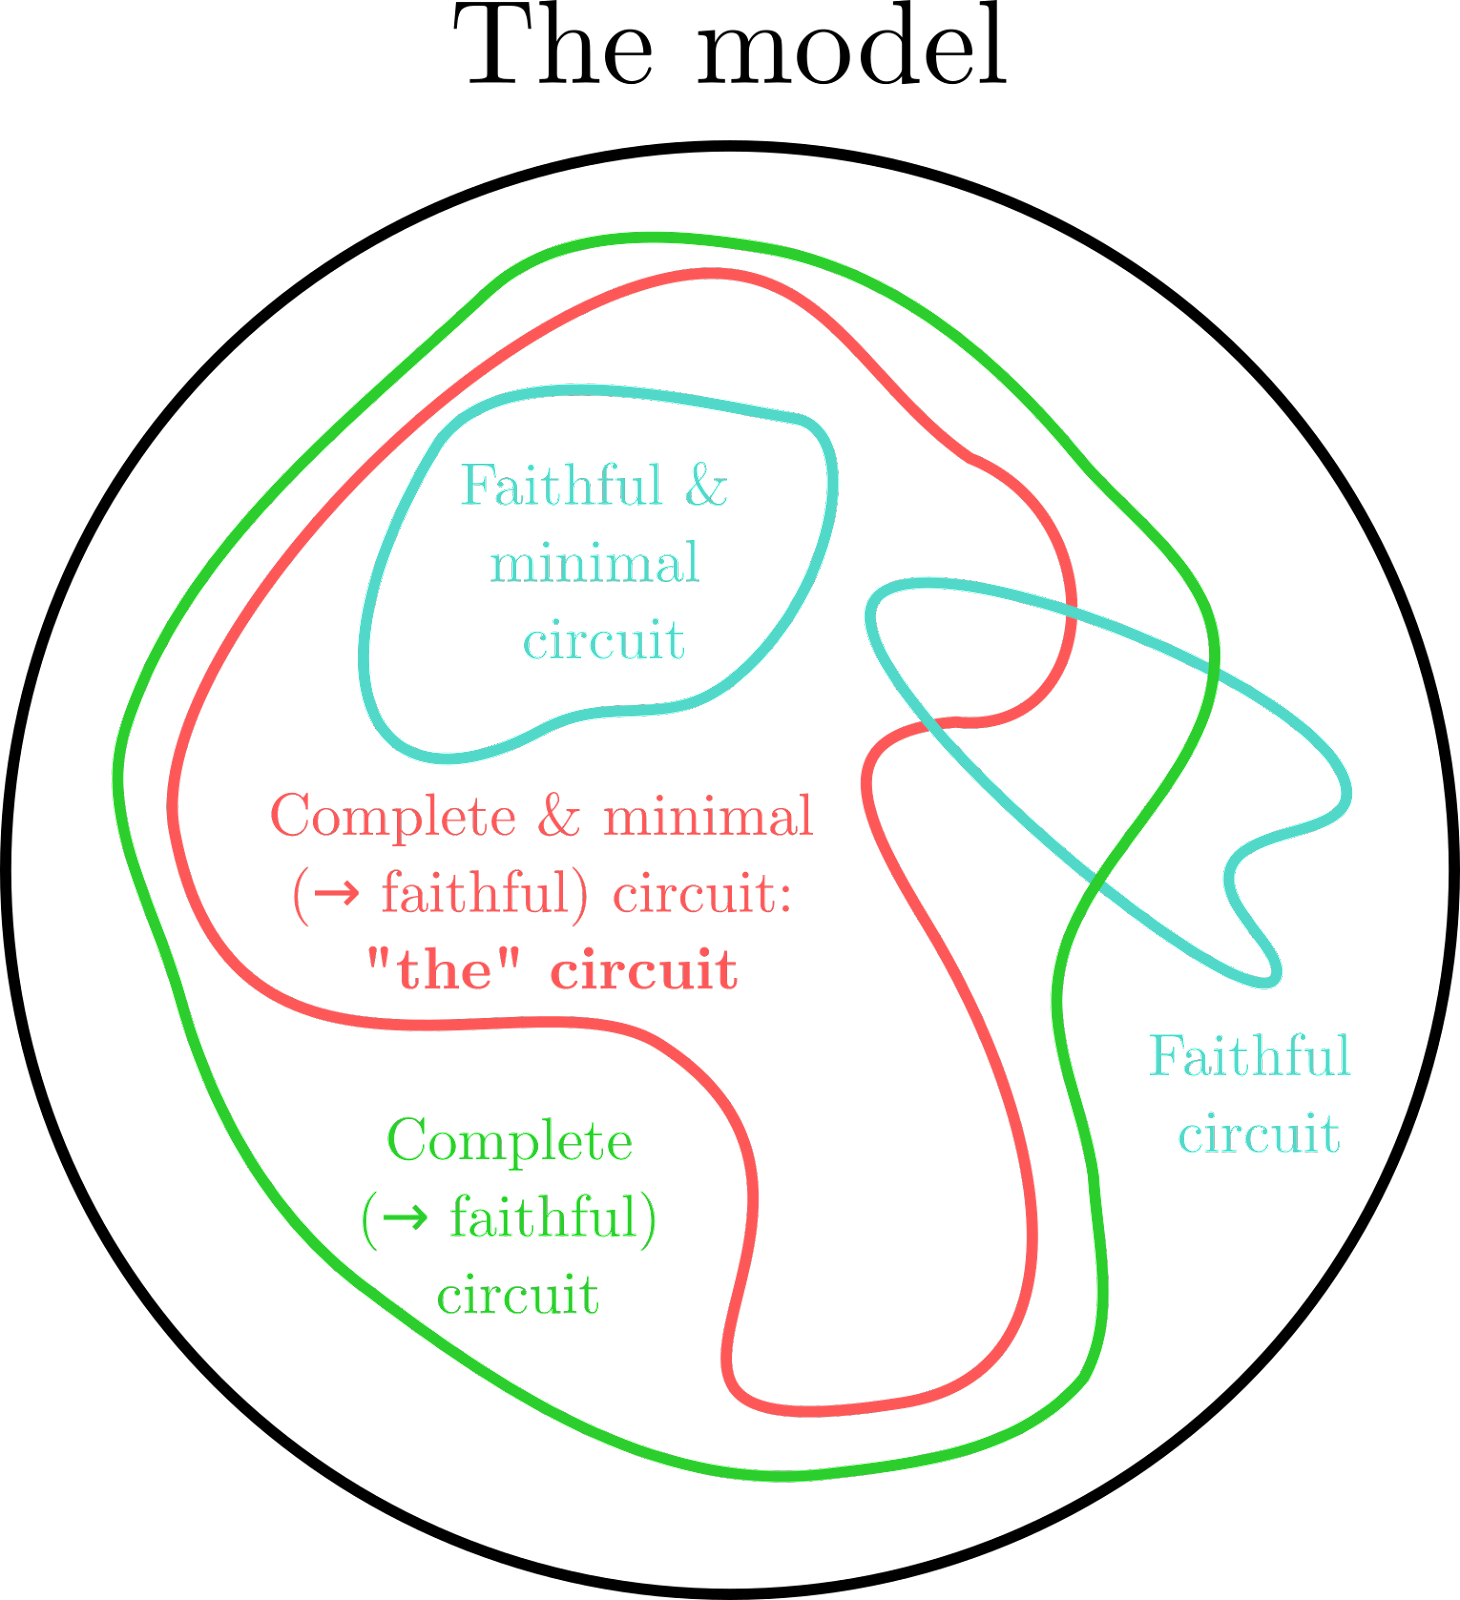
\includegraphics[width=0.4\textwidth]{figs/circuit_decomposition.png}
% \end{center}
% \caption{Illustration of possible circuits that could be found as subsets of the model's nodes.}
% \end{wrapfigure}

% \begin{itemize}
%     \item \textbf{Completeness}: our circuit is complete if it includes all the circuits that compute the task. We formulate this criterion by ensuring that if we remove certain nodes of the circuit, no part of the model can replace their effect on $F$. $\forall J \subseteq C, |\mathrm{F}(C \setminus J) - \mathrm{F}(M \setminus J)| \leq \epsilon$.
%     \item \textbf{Minimality}: our circuit is minimal if it does not include any nodes that are irrelevant for the task. Formally, for each node $v$ we have to find a subcircuit $J$ of $C$, such that when $v$ is added back in to $C\setminus J$, it makes a significant impact on $F$. $\forall v \in C, \exists J \subseteq C, |\mathrm{F}( (C \setminus J) \cup \{v\}) - \mathrm{F}( (C\setminus J))| \geq A$.
%     \item \textbf{Legibility}: our circuit is legible if the components in our circuit cleanly correspond to a human understandable causal model. In this work, we consider this to be a more qualitative evaluation from different metric of composition and causal intervention described above. 
% \end{itemize}

% We defined this framework to be reasonably rigorous while enabling an empirical evaluation of the proposed criteria. We chose to work with nodes instead of links to limit the combinatorial explosion of elements to investigate while ensuring a reasonable level of understanding. Moreover, the metric $F$ is used as a proxy for the behavior. In general, the task to understand contains different aspect that cannot be summarized in a single function. To validate our work, we choose several different $F$ and verify the criteria for each of them.
 
%We chose these criteria as a first attempt to ensure empirical evaluation of complex task in language models, future work could try to apply this approach with a more fine-grain mapping from the explanation to the model internals (see \ref{sec:future}).

% practical implem

% completness: adversarial approch
% minimality: certificat approach

%\todo{Talk about the baseline circuit}

% \subsection{Implementation of the explanation criteria}

% \subsubsection{Circuit definition}

% In full generality, we could consider each node of the computational graph implemented by a transformer as a succession of matrix multiplication and non-linear function. However, we used a more coarse-grained modelisation to express our empirical findings. More precisely, we are interested in understanding the mechanism responsible for information moving across token position. Attention heads are the units responsible for this role, this is why we consider nodes as being pairs $(h, \text{IND})$ where $h$ is an attention head and $\text{IND}$ a token position, as describe in the section \ref{sec:ablation}. The MLP and LayerNorm are not part of the computational circuit we consider. Those modules are always fully functional in our validation experiments. We also motivate this choice in appendix \ref{app:mlp} where we present several experiments suggesting a minimal role of the MLP for the IOI task.

% For $F$, we generally use the average logit difference (see section \ref{sec:metrics}), though verify our explanations are not too dependent on this metric by checking the IO probabilities, too.

% \subsubsection{Circuit extraction}

% The computational graph abstraction as introduced in section \ref{sec:explanation} cannot be naively transposed to transformers. In particular, for a circuit $C\subseteq M$, computing $F(C)$ by excluding every node from $M\setminus C$ is equivalent to perform zero-ablation on those nodes. This is surely not a great way to represent the absence of features from $M\setminus C$, as a zero activation is likely to be far from the natural computation and introduced corrupted computation in latter nodes. \ac{can't this section just cite \ref{sec:ablation} / that section cite this section? I don't think both are needed}

% To counteract these effects, we used in-template mean ablation to perform \emph{circuit extraction}. We build a circuit $C$ from $M$, by in-template mean ablating every node $(h, \text{IND}) \in M\setminus C$. This as for effect to remove the values of tokens in a particular sentence (e.g. the fact that the indirect object is `John`) while preserving the features linked to the structure of the sentence and the token position (e.g. the fact that the second token is a name). 

% Those restriction can be perceived as too permissive, however as we show in section \ref{sec:circuit_extr_validation} they preserve a significant amount of specificity. We show that a faithful and legible circuit that doesn't seem to miss any part to fully explain the behavior can fail our minimality and completeness test. This demonstrates that our technique is an effective way to evaluate explanation beyond appearances. This technique also enable to clearly define the scope of the investigation and could enable an incremental study of circuits by dividing the interpretability approach into tractable sub-goals that can be rigorously validated.

% \subsubsection{Set search}

% The definition of minimality and completeness described in \ref{sec:criteria} rely on an exhaustive search among subset of the circuit. Such an exhaustive search is not computationally tractable. 

% \textbf{Completeness} 
% A first approach is to use the division of heads into classes. Because classes perform similar function, removing them from the model is likely to identify node in $M\setminus C$ that could replace them.


% Alternatively, to ensure that $\forall J \subseteq C, |\mathrm{F}(C \setminus J) - \mathrm{F}(M \setminus J)| \leq \epsilon$ we can an adversarial approach against the circuit $C$ by greedily optimizing for $J$ node by node to maximize $|\mathrm{F}(C \setminus J) - \mathrm{F}(M \setminus J)|$. \av{Add the pseudo-code ? not the most intresting but can be included in appendix}
% This method gives us a lower bound on the actual completeness score that depends on the quality of the greedy search. However, we empirically found that the greedy search performed better than the approach by class making us confident that it is able to find good proxy for the global optimum.

% \textbf{Minimality} 
% The minimality criterion only require us to exhibit for every $v$ a certificate set $J$ such that $|\mathrm{F}( (C \setminus J) \cup \{v\}) - \mathrm{F}( (C\setminus J))| \geq A$. Again, most of the time this certificate can be guessed from the organization by class. If we remove the class of head $G$ and consider $C \setminus G$ with $v \in G$, it is likely that $|\mathrm{F}( (C \setminus G) \cup \{v\}) - \mathrm{F}( (C\setminus G))|$ will be significant is $v$ is able to partially recover the function of the class $G$ and if $\mathrm(F)(C)$ depend on this ability.
% \label{sec:criteria}